\section{Excedente del productos y del consumidor}
\begin{itemize}
    \item Asumir que estamos en equilibrio.
    \item Excedente del consumidor:
        \[
          C_S = \int_{0}^{Q*}\left[P(Q^D)-P*\right]dQ^D
        \]
    
    \item Excedente del productor:
        \[
          P_S = \int_{0}^{Q*}\left[ P*-P(Q^s) \right] dQ^s
        \]
    
    \item Excedente del consumidor y productor:
        \begin{figure}[!htb]
            \centering
            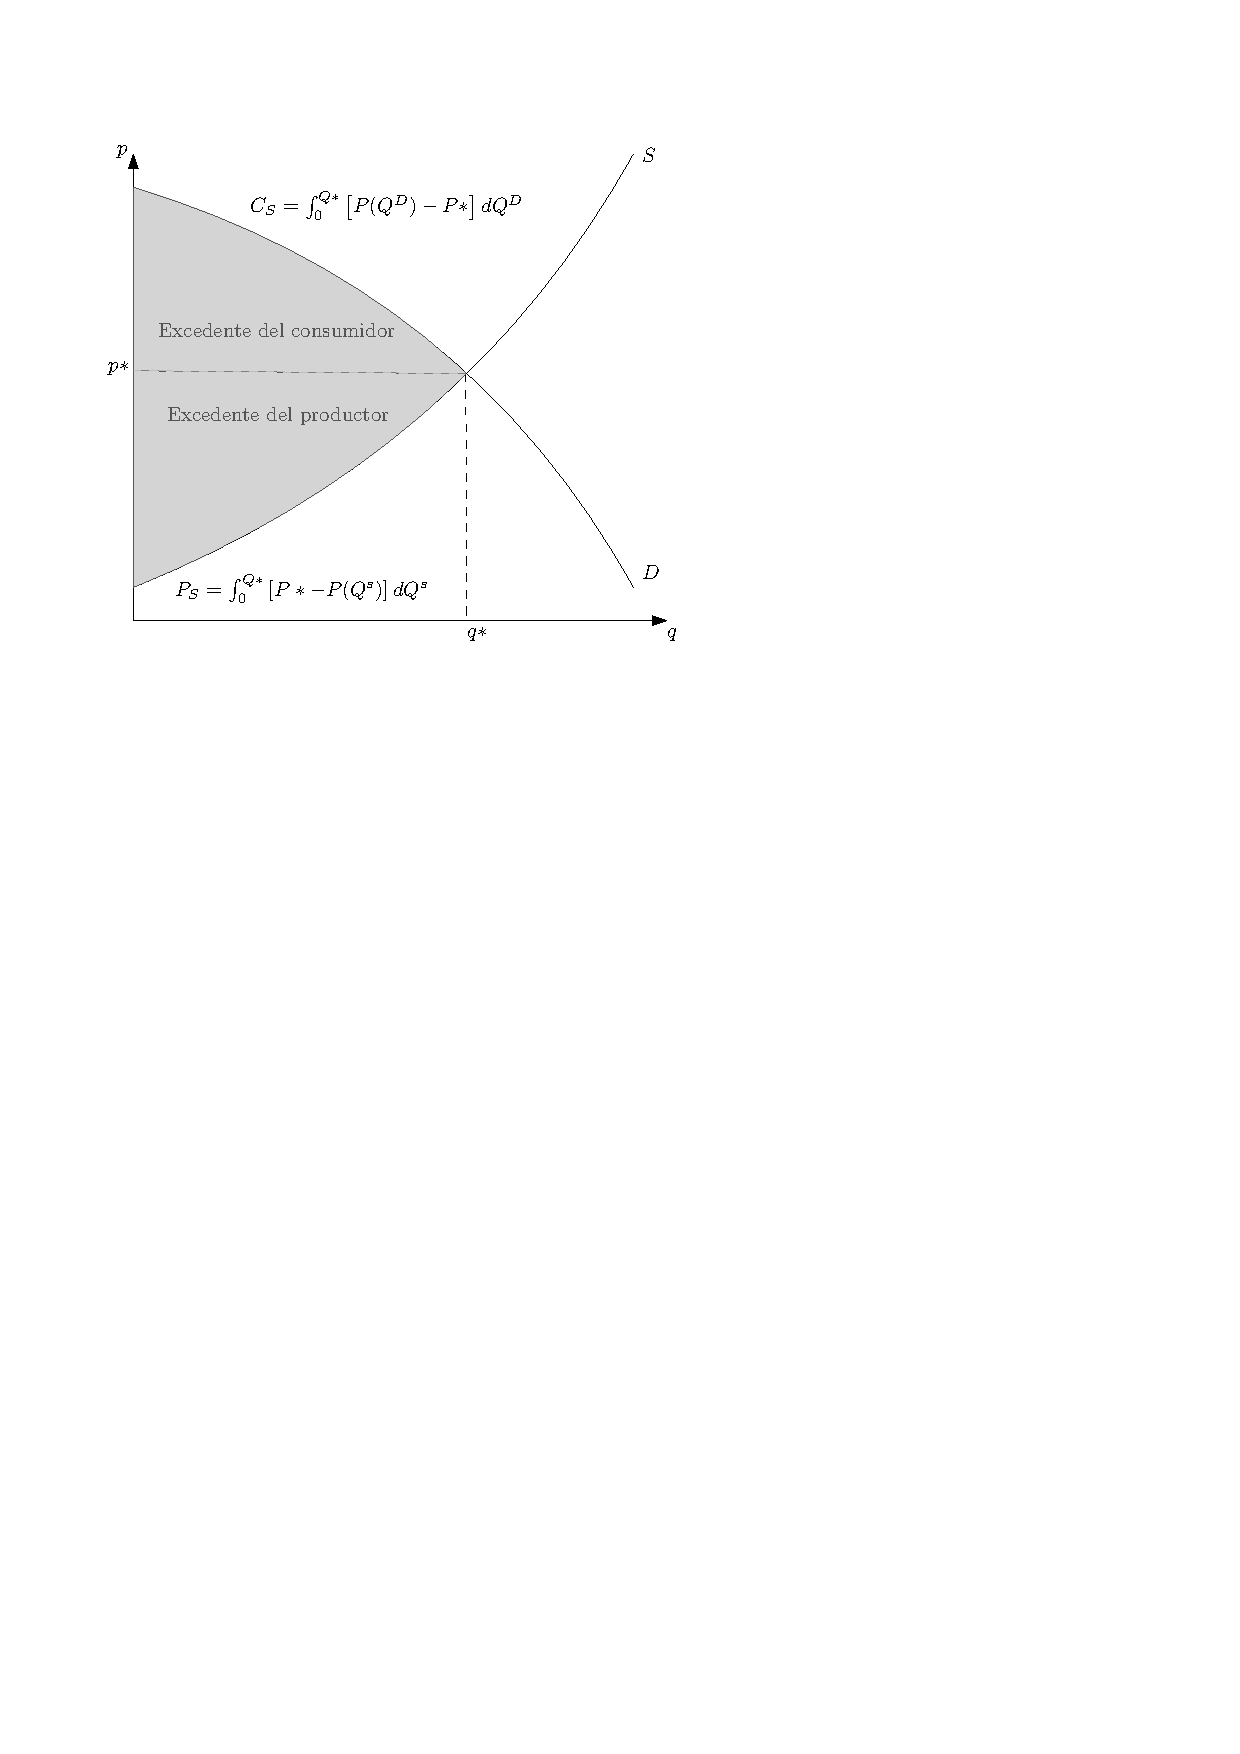
\includegraphics{Clases/figs/03}
        \end{figure}
    
    \item Precio máximo: El precio máximo está por debajo de equilibrio: $\displaystyle P_C < P*$ $\displaystyle Q_C$ es la cantidad vendida al precio máximo y $\displaystyle P_C$ es el precio máximo. 
        \[
          C_{S_C} = \int_{0}^{Q_c}\sqb{P\p{Q^D} -P_C} dQ^{\square}
        \]
        \[
          P_{S_C} = \int_{0}^{Q_C} \sqb{P_C-P\p{Q^S} } dQ^{\square}
        \]
        \begin{figure}[!htb]
            \centering
            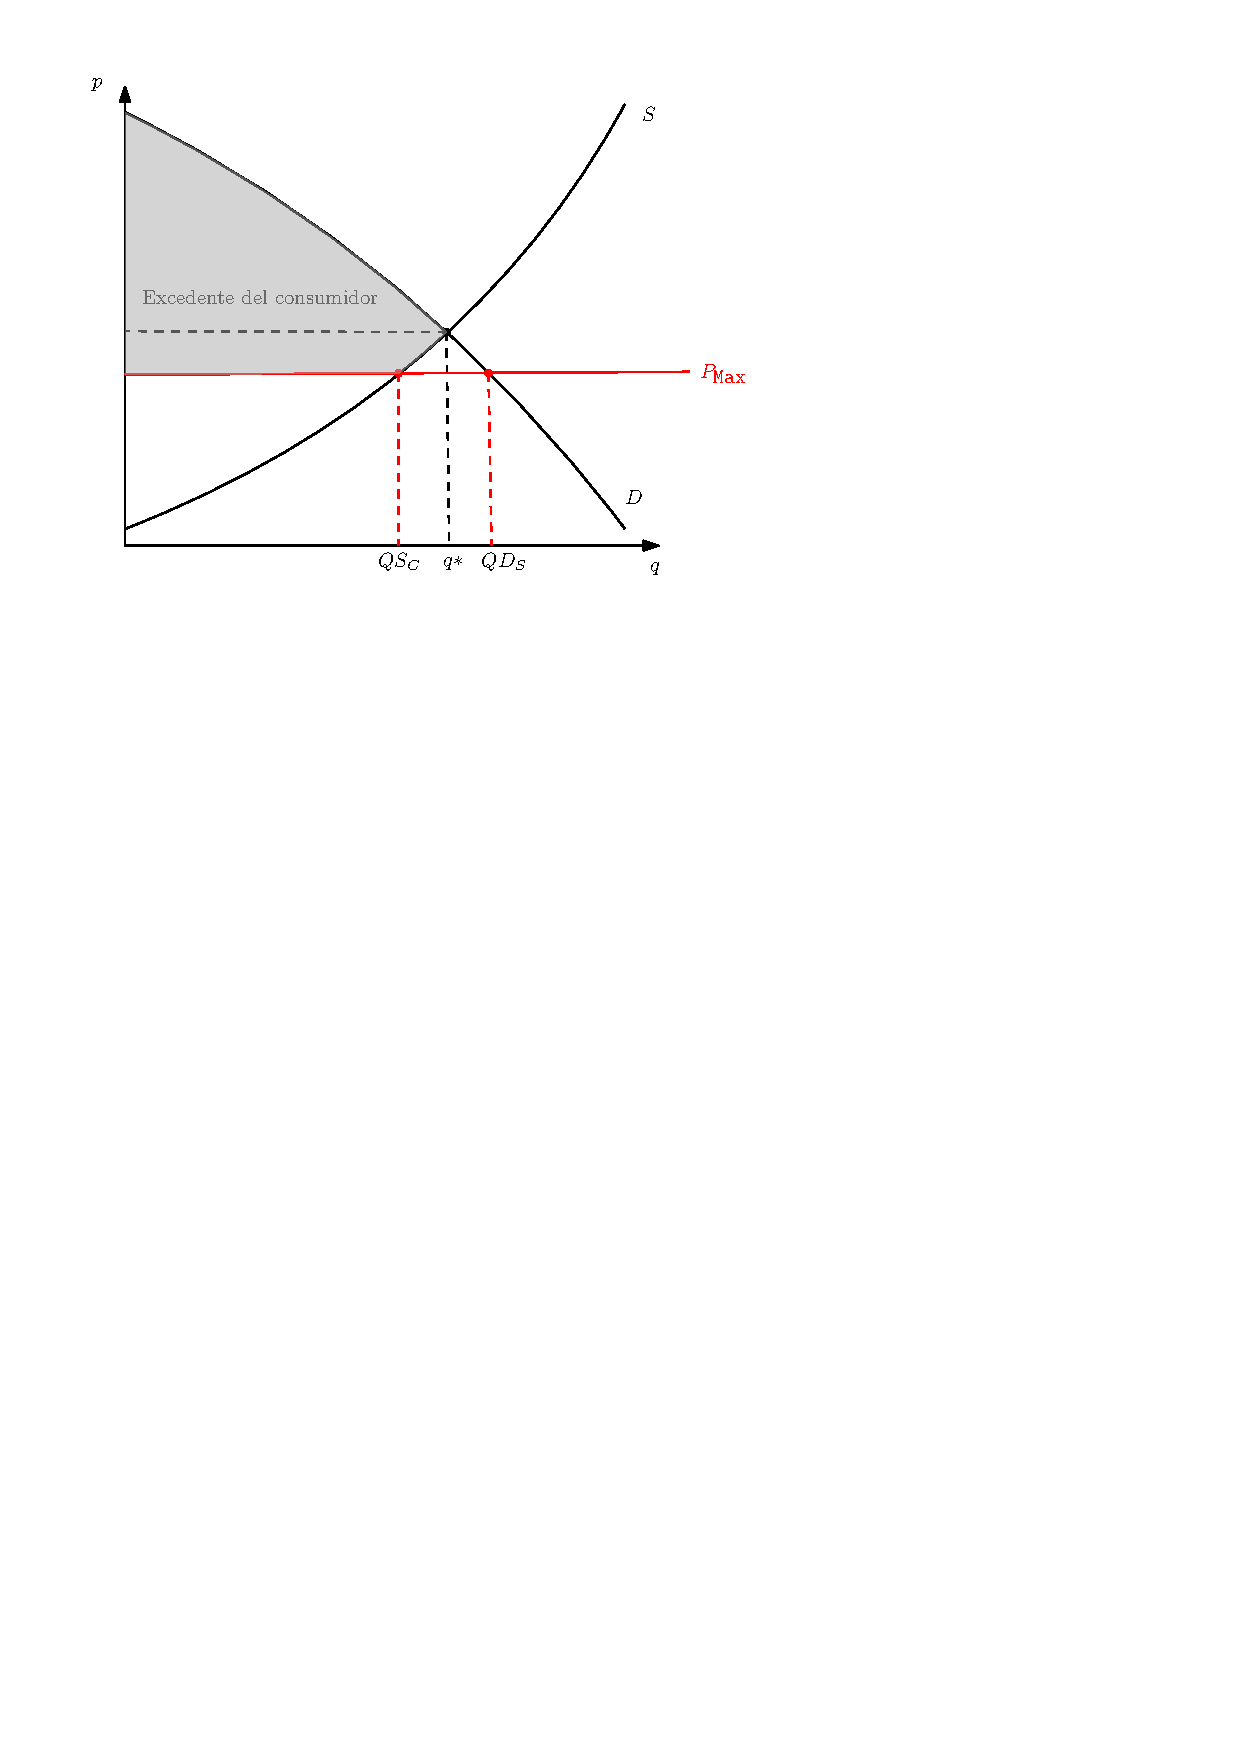
\includegraphics{Clases/figs/05}
        \end{figure}
    
    \item Precio mínimo: El precio mínimo estpa porarriba del precio de equilibrio: $\displaystyle P_f > P*$ y $\displaystyle Q_f$ es la cantidad demandada con el precio mínimo. $\displaystyle P_f$ es el precio mínimo.  
        \begin{figure}[!htb]
            \centering
            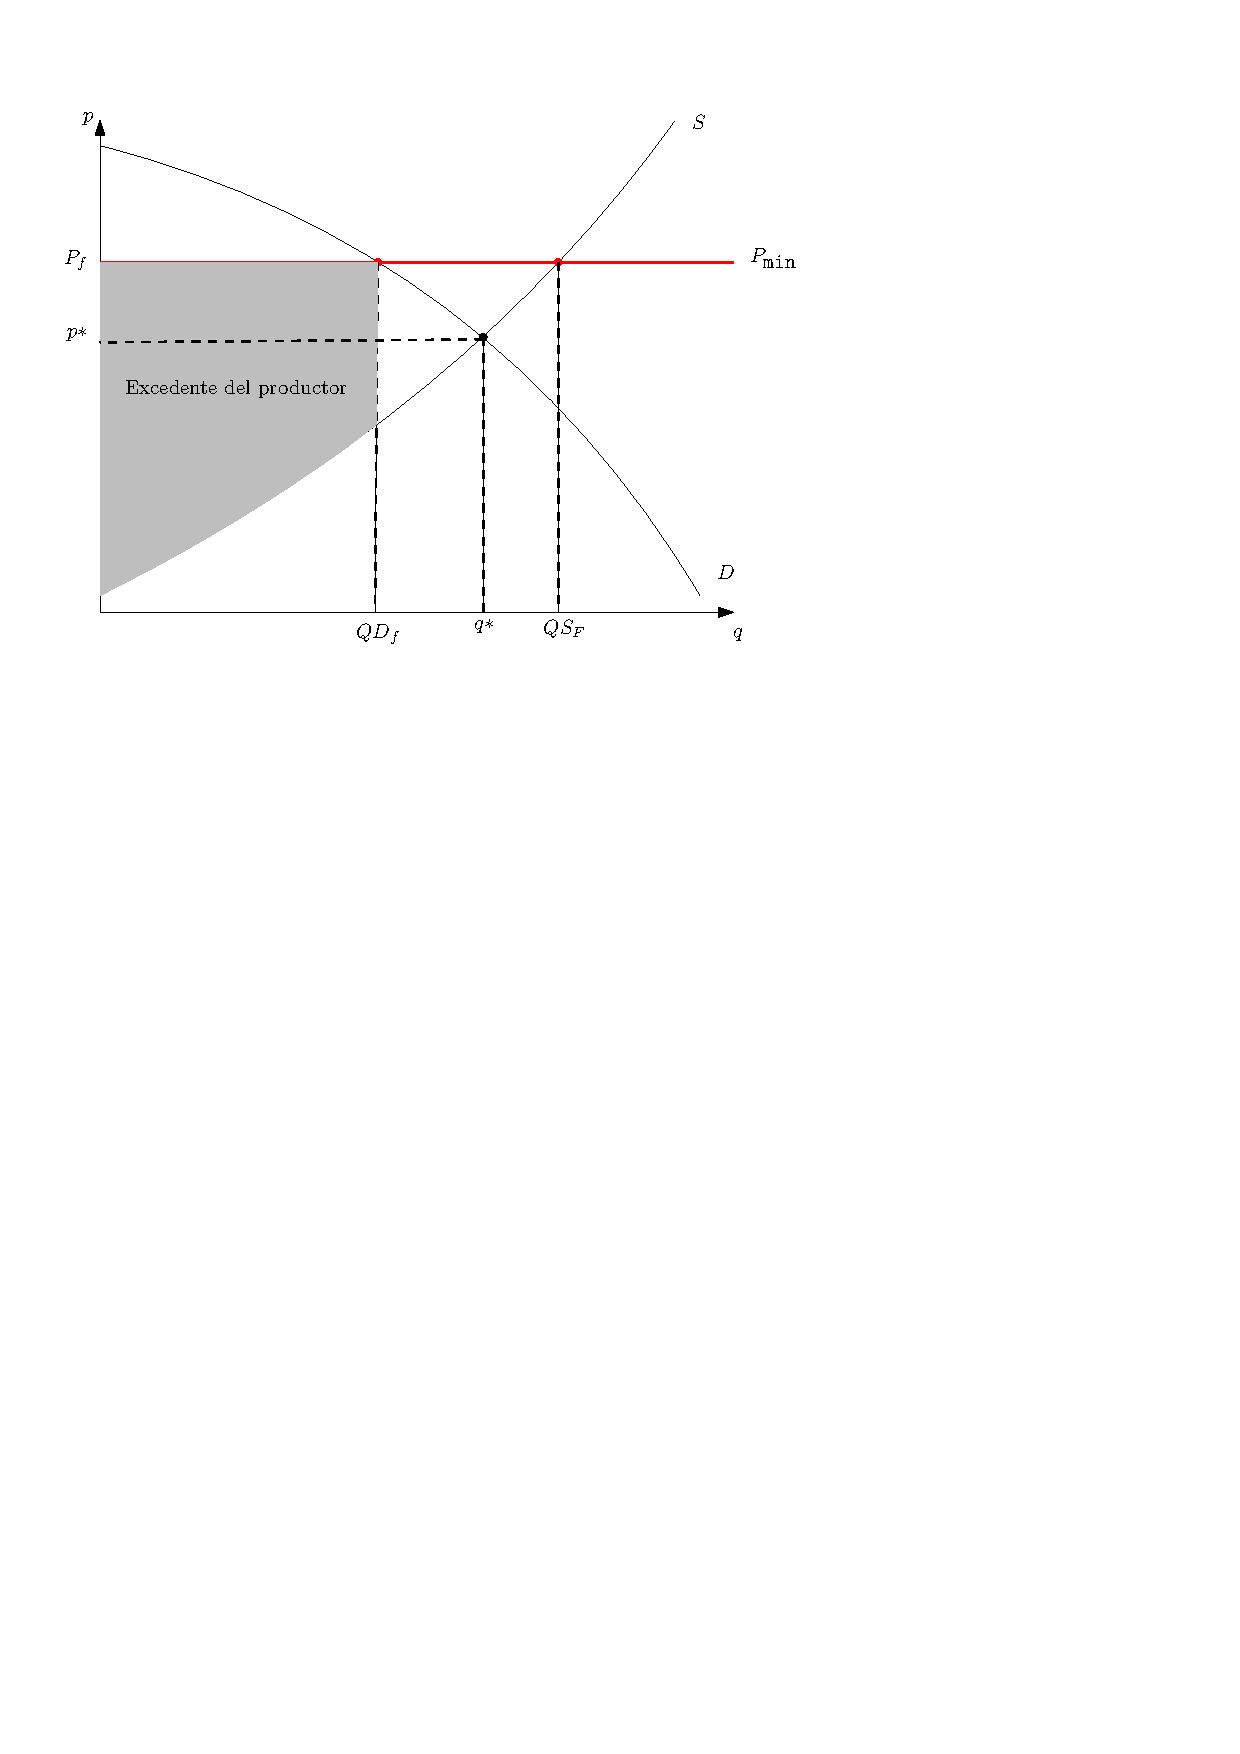
\includegraphics[]{Clases/figs/04} 
        \end{figure}
        
    \item Impuestos: 
        \begin{figure}[!htb]
            \centering
            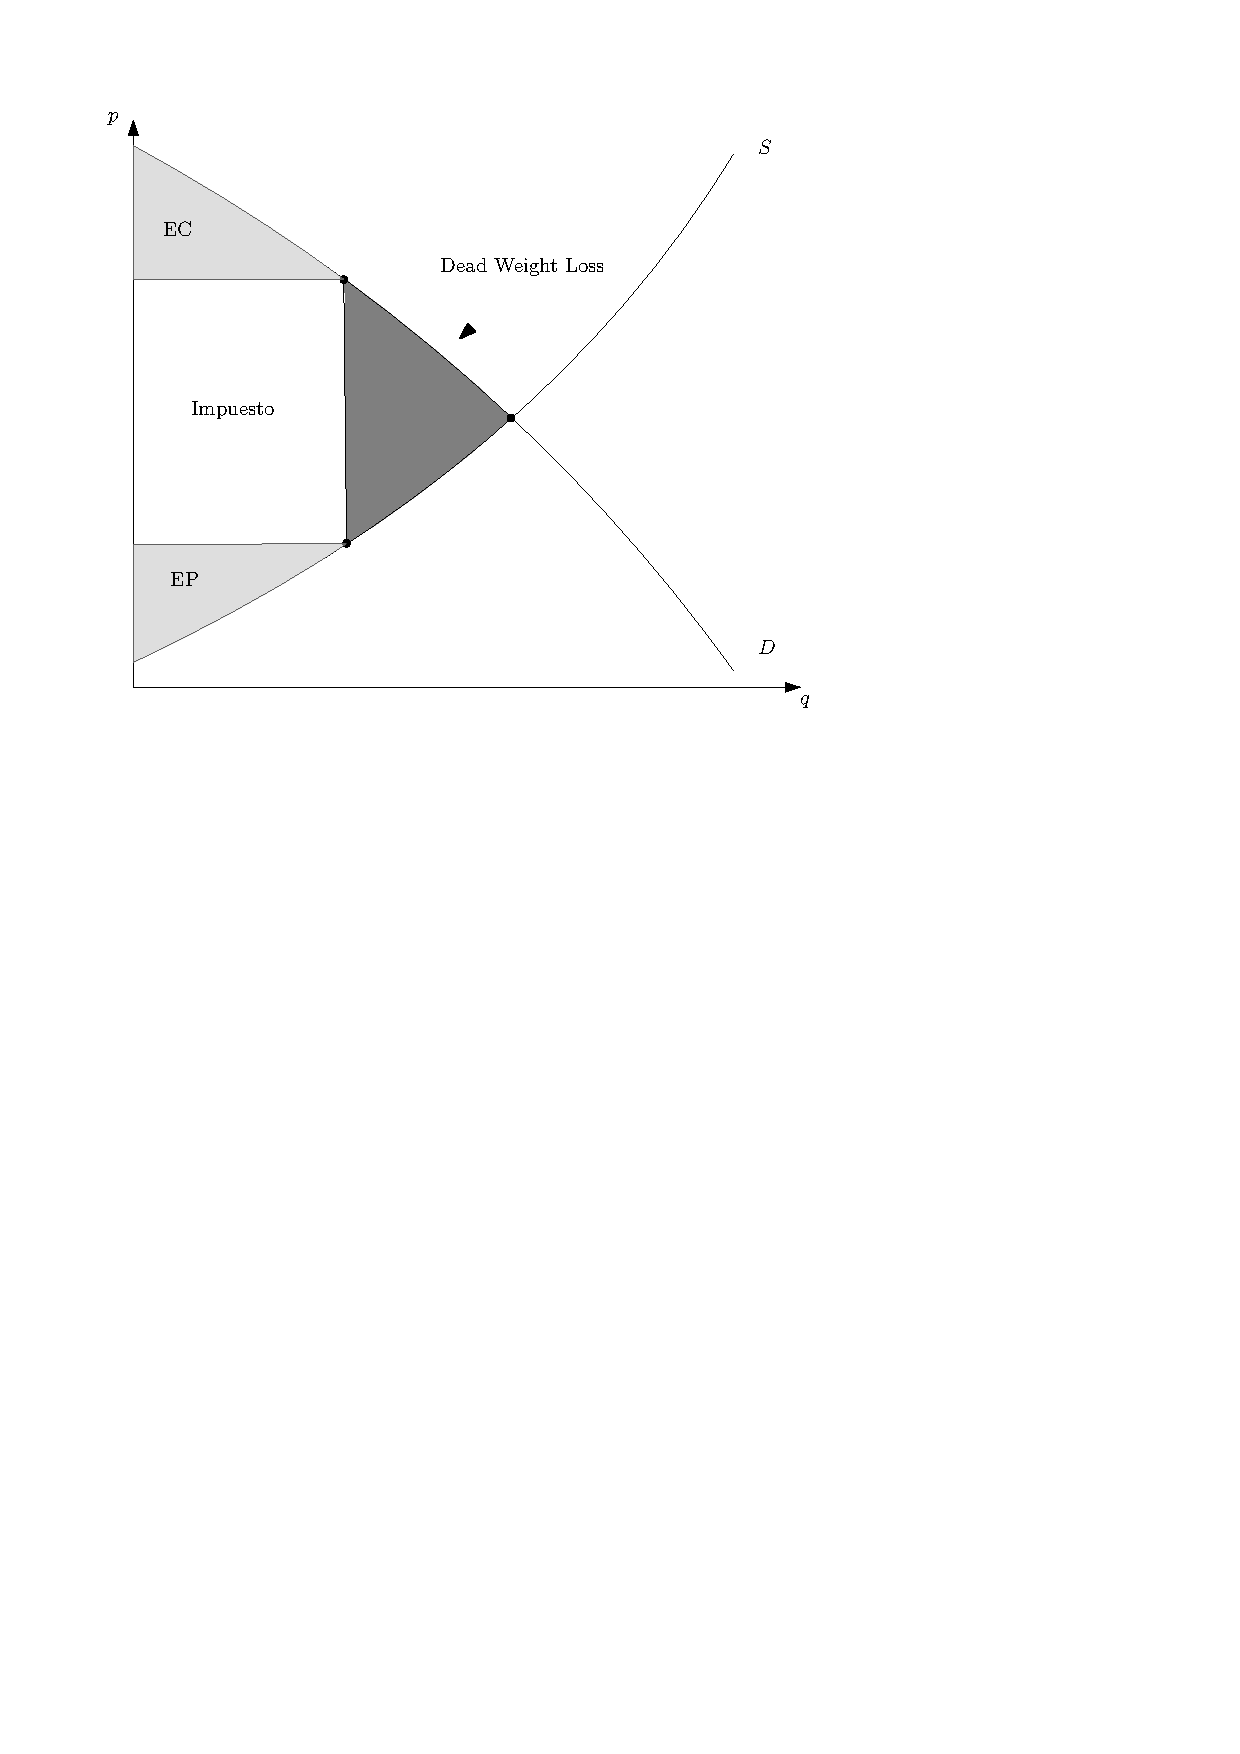
\includegraphics[]{Clases/figs/06} 
        \end{figure}
\end{itemize}


%----------------------------------------------------------------------------------------
\subsection{Ejercicio}
\begin{itemize}
    \item Demanda de Widgets: $\displaystyle D(q) = 200-q^2$ Oferta: $\displaystyle S(q) = q^2+38$, Encontrar CS y PS:  
        \begin{center}
           \begin{align*}
               q* = 9 \qq & \qq p*=119 \\ 
               C_S &= \int_{0}^{9}\p{200-q^2-119} dq \\ 
                &= 200q-\frac{q^3}{3} -119q \qq \evaluate{0}{9} \\ 
                & = \text{ \$ }486 \\ 
           \end{align*}
        \end{center}
\end{itemize}
